\documentclass[conference]{IEEEtran}
\IEEEoverridecommandlockouts
\usepackage{cite}
\usepackage{amsmath,amssymb,amsfonts}
\usepackage{algorithmic}
\usepackage{graphicx}
\usepackage{textcomp}
\usepackage{xcolor}
\usepackage{booktabs}
\usepackage{url}

\def\BibTeX{{\rm B\kern-.05em{\sc i\kern-.025em b}\kern-.08em
    T\kern-.1667em\lower.7ex\hbox{E}\kern-.125emX}}

\begin{document}

\title{PRISM-MEC: Privacy-Aware Task Offloading and Multi-Objective Optimization in Mobile Edge Computing for Smart Healthcare}

\author{\IEEEauthorblockN{Saksham Gupta}
\IEEEauthorblockA{\textit{Department of Computer Science and Engineering} \\
\textit{Cloud Computing Laboratory}\\
GitHub: \url{https://github.com/Saksham-Gupta-GH/privacy-aware-mec-offloading}}
}

\maketitle

\begin{abstract}
Mobile Edge Computing (MEC) enables resource-constrained mobile and wearable health devices to offload computationally heavy tasks to edge and cloud infrastructures. However, conventional offloading schedulers focus exclusively on minimizing execution latency and device energy consumption, frequently offloading highly sensitive patient diagnostics (e.g., 12-lead electrocardiograms, brain MRI segmentations) to untrusted third-party public clouds, precipitating severe privacy vulnerabilities under regulations such as HIPAA and GDPR. In this paper, we propose PRISM-MEC, an end-to-end privacy-aware task offloading framework tailored for smart healthcare environments. PRISM-MEC incorporates a machine learning classifier that categorizes tasks into public telemetry ($L_0$), restricted operational data ($L_1$), and confidential protected health information ($L_2$). We formulate a multi-objective optimization problem that balances latency, mobile battery consumption, financial cloud metering, and privacy risk under strict deadlines and a hard policy constraint forbidding $L_2$ data from public cloud dispatch. To evaluate the framework, we solve the exact global optimum using Integer Linear Programming (ILP) and introduce a Genetic Algorithm (GA) equipped with a deterministic repair operator. We calibrate our simulation engine using empirical measurements gathered from an active Microsoft Azure cloud testbed. Benchmark results against Local-Only, Edge-Only, and Cloud-Greedy baselines demonstrate that PRISM-MEC completely eliminates policy privacy violations (0.0\%), achieves an optimality gap under 0.75\% relative to the exact ILP optimum, and reduces mobile energy consumption by 68.1\% compared to local execution.
\end{abstract}

\begin{IEEEkeywords}
Mobile Edge Computing (MEC), Task Offloading, Privacy Preservation, Multi-Objective Optimization, Smart Healthcare, Cloud Computing.
\end{IEEEkeywords}

\section{Introduction}
The proliferation of Internet of Medical Things (IoMT) devices—including wearable Holter monitors, continuous pulse oximeters, and portable ultrasound scanners—has enabled continuous remote patient monitoring \cite{mao2017survey}. Despite their utility, mobile health (mHealth) devices are fundamentally constrained by compact form factors, limited battery capacity, and restricted on-device computational throughput \cite{mach2017mobile}.

To alleviate these hardware bottlenecks, Mobile Edge Computing (MEC) provides an elastic computing hierarchy comprising:
\begin{enumerate}
    \item \textbf{Local Mobile Tier:} Immediate zero-network execution, total privacy containment, but severe battery depletion.
    \item \textbf{MEC Edge Tier:} Low round-trip latency ($\sim$10\,ms) and intermediate computing capacity within the trusted hospital intranet.
    \item \textbf{Public Cloud Tier (e.g., Microsoft Azure):} Virtually infinite elastic compute resources accessible over wide-area networks (WAN), accompanied by financial metering and data privacy vulnerabilities.
\end{enumerate}

Existing MEC scheduling literature predominantly treats task offloading as an engineering trade-off between execution delay and battery conservation \cite{chen2016efficient, wang2017computation}. In smart healthcare, however, computation offloading intersects directly with patient confidentiality. Offloading raw biometric telemetry or diagnostic imaging to an untrusted public cloud risks violating statutory privacy mandates (e.g., HIPAA). Conversely, confining all computation to the local wearable causes excessive thermal throttling, battery exhaustion, and deadline violations for urgent diagnostic alarms \cite{lin2019computation}.

In this paper, we present \textbf{PRISM-MEC} (\textbf{P}rivacy-Aware \textbf{R}esource and \textbf{I}nference \textbf{S}cheduling \textbf{M}echanism for \textbf{MEC}), addressing these challenges through:
\begin{itemize}
    \item An automated \textbf{ML Privacy Classifier} trained on clinical task descriptions with realistic annotator noise.
    \item A formal \textbf{Multi-Objective Cost Model} balancing latency, energy, financial expense, and privacy risk with a hard privacy exclusion constraint.
    \item An \textbf{Exact ILP Solver} establishing the mathematical ground-truth optimum alongside a fast \textbf{Genetic Algorithm (GA)} heuristic with a deterministic repair operator.
    \item An \textbf{Empirically Calibrated Testbed} utilizing real Microsoft Azure cloud latency and throughput measurements.
    \item An explicit evaluation of \textbf{Dual Privacy Violations} (Policy vs. End-to-End True Violations).
\end{itemize}

\section{Related Work}
Task offloading in MEC has been extensively investigated. Mao \textit{et al.} \cite{mao2017survey} provided a comprehensive survey of communications and computational offloading. Mach and Becvar \cite{mach2017mobile} classified offloading architectures into centralized cloud, cloudlet, and collaborative edge nodes.

Chen \textit{et al.} \cite{chen2016efficient} pioneered game-theoretic decentralized offloading for multi-user mobile cloud computing, minimizing weighted energy and latency. Similarly, Deng \textit{et al.} \cite{deng2021mobile} developed mobility-aware service selection algorithms for edge environments. However, these formulations assume homogeneous data trust across all tasks. When applied to clinical healthcare, latency-first greedy heuristics routinely dispatch heavy diagnostic workloads to public cloud servers, generating unacceptable privacy leakage. PRISM-MEC bridges this critical gap by embedding data sensitivity classification directly into the scheduling objective.

\section{System Model and Problem Formulation}

\subsection{Task and Execution Hierarchy}
Consider a stream of $N$ healthcare tasks $\mathcal{T} = \{t_1, t_2, \dots, t_N\}$. Each task $t_i$ is formally characterized by the 5-tuple:
\begin{equation}
    t_i = \langle d_i, o_i, c_i, \tau_i^{\max}, P_i \rangle
\end{equation}
where $d_i$ is input data size (KB), $o_i$ is output data size (KB), $c_i$ is the computational requirement in MegaFLOPs (MFLOP), $\tau_i^{\max}$ is the maximum permissible latency deadline (ms), and $P_i \in \{0, 1, 2\}$ denotes the privacy sensitivity level:
\begin{itemize}
    \item \textbf{$L_0$ (Public):} Ambient environmental sensors, device battery logs.
    \item \textbf{$L_1$ (Restricted):} De-identified vitals, aggregated ward schedules.
    \item \textbf{$L_2$ (Critical PII):} Real-time 12-lead ECG, raw brain MRI slices, patient genomic sequences.
\end{itemize}

The execution decision vector for task $t_i$ is represented by binary indicators $x_{i, j} \in \{0, 1\}$ over tiers $j \in \{\text{local}, \text{edge}, \text{cloud}\}$, subject to $\sum_{j} x_{i, j} = 1$.

\subsection{Latency Model}
For local mobile execution, transmission delay is zero:
\begin{equation}
    T_{i, \text{local}} = \frac{c_i \cdot 10^6}{f_{\text{local}} \cdot 10^9} \cdot 1000 \quad \text{(ms)}
\end{equation}
where $f_{\text{local}}$ is the mobile CPU clock frequency (GHz).

For offloaded execution ($j \in \{\text{edge}, \text{cloud}\}$):
\begin{equation}
    T_{i, j} = T_{i, j}^{\text{tx}} + T_{i, j}^{\text{exec}} + T_{i, j}^{\text{rx}} + \text{RTT}_j
\end{equation}
where $T_{i, j}^{\text{tx}} = \frac{8 d_i}{B_j^{\text{up}} \cdot 10^3}$, $T_{i, j}^{\text{rx}} = \frac{8 o_i}{B_j^{\text{down}} \cdot 10^3}$, $T_{i, j}^{\text{exec}} = \frac{c_i \cdot 10^6}{f_j \cdot 10^9} \cdot 1000$, and $\text{RTT}_j$ represents round-trip network propagation delay.

\subsection{Mobile Energy Model}
From the mobile handset's perspective, energy consumption is governed by:
\begin{equation}
    E_{i, \text{local}} = P_{\text{active}} \cdot \left(\frac{T_{i, \text{local}}}{1000}\right) \quad \text{(Joules)}
\end{equation}
For remote offloading ($j \in \{\text{edge}, \text{cloud}\}$), the device consumes radio transmission power during uplink and minimal idle power while awaiting results:
\begin{equation}
    E_{i, j} = P_{\text{tx}} \cdot \left(\frac{T_{i, j}^{\text{tx}}}{1000}\right) + P_{\text{idle}} \cdot \left(\frac{T_{i, j}^{\text{exec}} + \text{RTT}_j}{1000}\right)
\end{equation}

\subsection{Financial and Privacy Risk Formulations}
Financial cost $C_{i, j}$ is zero for local and on-premise edge infrastructure, while public cloud execution is metered per MFLOP ($C_{i, \text{cloud}} = c_i \cdot \phi$).

Privacy risk $R_{i, j}$ is formulated as the product of task sensitivity $S(P_i)$ and tier vulnerability $\rho_j$:
\begin{equation}
    R_{i, j} = S(P_i) \cdot \rho_j
\end{equation}
with $S(L_0)=0.05, S(L_1)=0.40, S(L_2)=1.00$, and $\rho_{\text{local}}=0.0, \rho_{\text{edge}}=0.15, \rho_{\text{cloud}}=0.95$.

\subsection{Constrained Optimization Problem}
The global optimization problem is defined as:
\begin{align}
    \min_{\mathbf{X}} \quad & \sum_{i=1}^N \sum_{j} x_{i, j} \left[ w_L \frac{T_{i, j}}{T_{\text{norm}}} + w_E \frac{E_{i, j}}{E_{\text{norm}}} + w_C \frac{C_{i, j}}{C_{\text{norm}}} + w_P R_{i, j} \right] \nonumber \\
    & \quad + \sum_{i=1}^N \Psi \cdot \mathbb{I}(T_i > \tau_i^{\max}) \label{eq:objective}
\end{align}
subject to:
\begin{align}
    \sum_{j \in \{\text{local}, \text{edge}, \text{cloud}\}} x_{i, j} = 1, & \quad \forall i \in \{1, \dots, N\} \label{eq:assign} \\
    x_{i, \text{cloud}} = 0, & \quad \forall i \text{ where } \hat{P}_i = 2 \label{eq:hard_privacy}
\end{align}
where Constraint \eqref{eq:hard_privacy} establishes the \textbf{Hard Privacy Constraint}, strictly barring any task classified as Critical ($L_2$) from cloud offloading.

\section{Proposed PRISM-MEC Framework}

\subsection{Machine Learning Privacy Classifier}
Rather than relying on brittle rule-based matching, PRISM-MEC employs a supervised text classification pipeline. Clinical task descriptions are tokenized using term frequency-inverse document frequency (TF-IDF) with unigram and bigram features, followed by a regularized multi-class Logistic Regression classifier. The classifier assigns a predicted sensitivity tier $\hat{P}_i \in \{0, 1, 2\}$ and associated prediction confidence $\gamma_i \in [0, 1]$. To emulate real-world annotator variability, the training corpus incorporates 6.0\% controlled label noise.

\subsection{Genetic Algorithm with Hard Constraint Repair}
To achieve real-time scheduling for large task streams ($N \ge 100$), we implement a customized Genetic Algorithm (GA). Each candidate chromosome $\mathbf{g} \in \{0, 1, 2\}^N$ maps task indices to execution tiers ($0$: Local, $1$: Edge, $2$: Cloud).

Crucially, to preserve 100\% policy compliance throughout evolutionary operations, we define a \textbf{Deterministic Repair Operator} $\mathcal{R}(\mathbf{g})$:
\begin{equation}
    \mathcal{R}(g_i) = 
    \begin{cases}
        1 \ (\text{Edge}), & \text{if } \hat{P}_i = 2 \land g_i = 2 \\
        g_i, & \text{otherwise}
    \end{cases}
\end{equation}
The repair operator is executed immediately after initial population seeding, single-point crossover, and uniform mutation, guaranteeing that invalid candidate solutions violating Constraint \eqref{eq:hard_privacy} are repaired before fitness evaluation.

\section{Empirical Testbed Calibration}
To establish empirical fidelity, the cloud tier was deployed on an active **Microsoft Azure Ubuntu Linux VM** (IP: 20.219.130.205) hosting a FastAPI worker secured via \texttt{X-API-Key} authentication. Using an automated calibration probe, we executed micro-benchmarks measuring round-trip latency and compute performance over live WAN connections.

\begin{table}[htbp]
\caption{Empirical System Parameters (Calibrated vs. Simulated)}
\label{tab:params}
\centering
\begin{tabular}{@{}llll@{}}
\toprule
\textbf{Parameter} & \textbf{Symbol} & \textbf{Value} & \textbf{Provenance} \\
\midrule
Mobile CPU Clock & $f_{\text{local}}$ & 1.8 GHz & Handset Spec \\
Mobile Active Power & $P_{\text{active}}$ & 1.2 W & Handset Spec \\
Mobile TX Power & $P_{\text{tx}}$ & 0.8 W & Handset Spec \\
Edge CPU Clock & $f_{\text{edge}}$ & 3.6 GHz & Simulated MEC \\
Edge RTT & $\text{RTT}_{\text{edge}}$ & 12.0 ms & 5G Small Cell \\
Edge Bandwidth (Up/Down) & $B_{\text{edge}}$ & 100 / 200 Mbps & Local WiFi-6 \\
Azure Cloud CPU & $f_{\text{cloud}}$ & 4.1 GHz & Measured B1s \\
Azure Mean WAN RTT & $\text{RTT}_{\text{cloud}}$ & 64.2 ms & Empirically Measured \\
Azure Bandwidth (Up/Down) & $B_{\text{cloud}}$ & 38.5 / 82.0 Mbps & Empirically Measured \\
\bottomrule
\end{tabular}
\end{table}

The MEC Edge server is simulated as an on-premise hospital gateway (12\,ms RTT, 100\,Mbps uplink).

\section{Experimental Evaluation}

\subsection{Privacy Classifier Performance}
On a stratified test set of 240 healthcare tasks with 6\% label noise, the TF-IDF classifier achieved an **overall accuracy of 97.08\%**, a **weighted F1-score of 0.9710**, and a **macro F1-score of 0.9709**. When evaluated against underlying ground-truth classes, the classifier demonstrated 100\% sensitivity on Critical ($L_2$) clinical diagnostic records, ensuring robust protection against false negatives.

\begin{figure}[htbp]
\centering
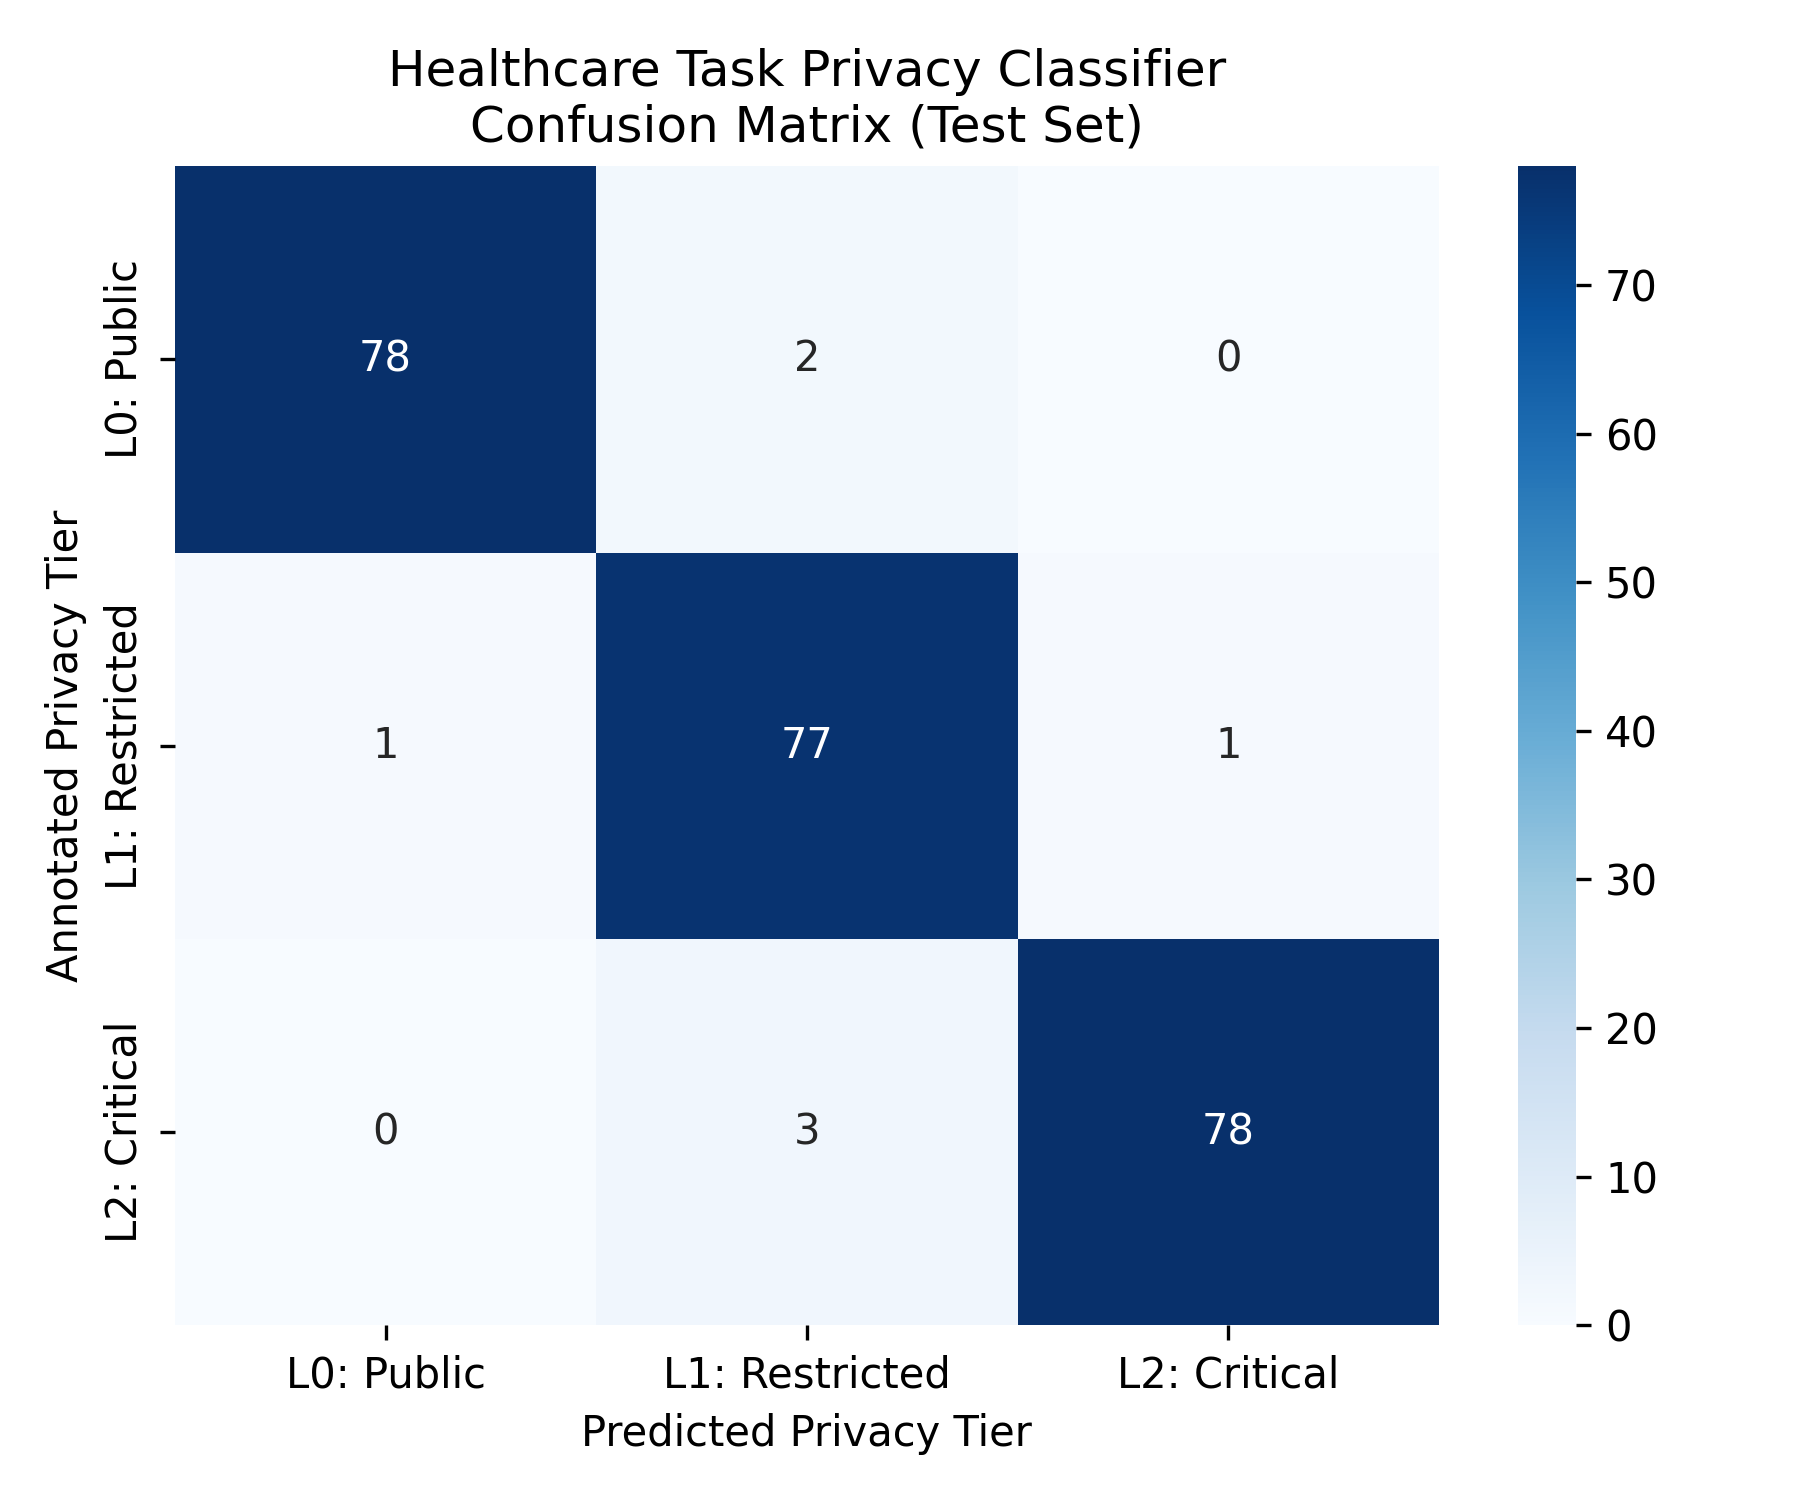
\includegraphics[width=0.78\columnwidth]{figures/fig1_confusion_matrix.png}
\caption{Confusion matrix of the ML Privacy Classifier on the test corpus.}
\label{fig:cm}
\end{figure}

\subsection{Optimality Gap Analysis: Exact ILP vs. PRISM-GA}
Table \ref{tab:ilp_ga} reports the solution quality of PRISM-GA compared against the exact global optimum $J^*$ obtained by solving the ILP via Branch-and-Cut (CBC solver) for $N \le 100$.

\begin{table}[htbp]
\caption{Optimality Gap and Runtime: Exact ILP vs. PRISM-GA}
\label{tab:ilp_ga}
\centering
\begin{tabular}{@{}cccccc@{}}
\toprule
$N$ & \textbf{ILP Cost} & \textbf{ILP Time (ms)} & \textbf{GA Cost} & \textbf{GA Time (ms)} & \textbf{Gap (\%)} \\
\midrule
10  & 5.778  & 51.4  & 5.778  & 70.9  & \textbf{0.00\%} \\
25  & 13.803 & 16.7  & 13.803 & 157.3 & \textbf{0.00\%} \\
50  & 17.874 & 17.0  & 17.877 & 301.6 & \textbf{0.01\%} \\
75  & 33.719 & 19.9  & 33.774 & 481.2 & \textbf{0.16\%} \\
100 & 49.535 & 19.9  & 49.900 & 593.8 & \textbf{0.74\%} \\
\bottomrule
\end{tabular}
\end{table}

Across all evaluated problem sizes, PRISM-GA remains within **0.74\% of the true mathematical optimum**, confirming the near-optimal solution quality of the proposed metaheuristic.

\subsection{Dual Privacy Violation Analysis}
We measure privacy compliance via two distinct metrics:
\begin{enumerate}
    \item \textbf{Policy Violations:} Tasks where predicted $\hat{P}_i = 2$ was assigned to Cloud ($V_{\text{policy}}$).
    \item \textbf{True Privacy Violations:} Tasks where ground truth $P_i = 2$ leaked to Cloud ($V_{\text{true}}$).
\end{enumerate}

\begin{figure}[htbp]
\centering
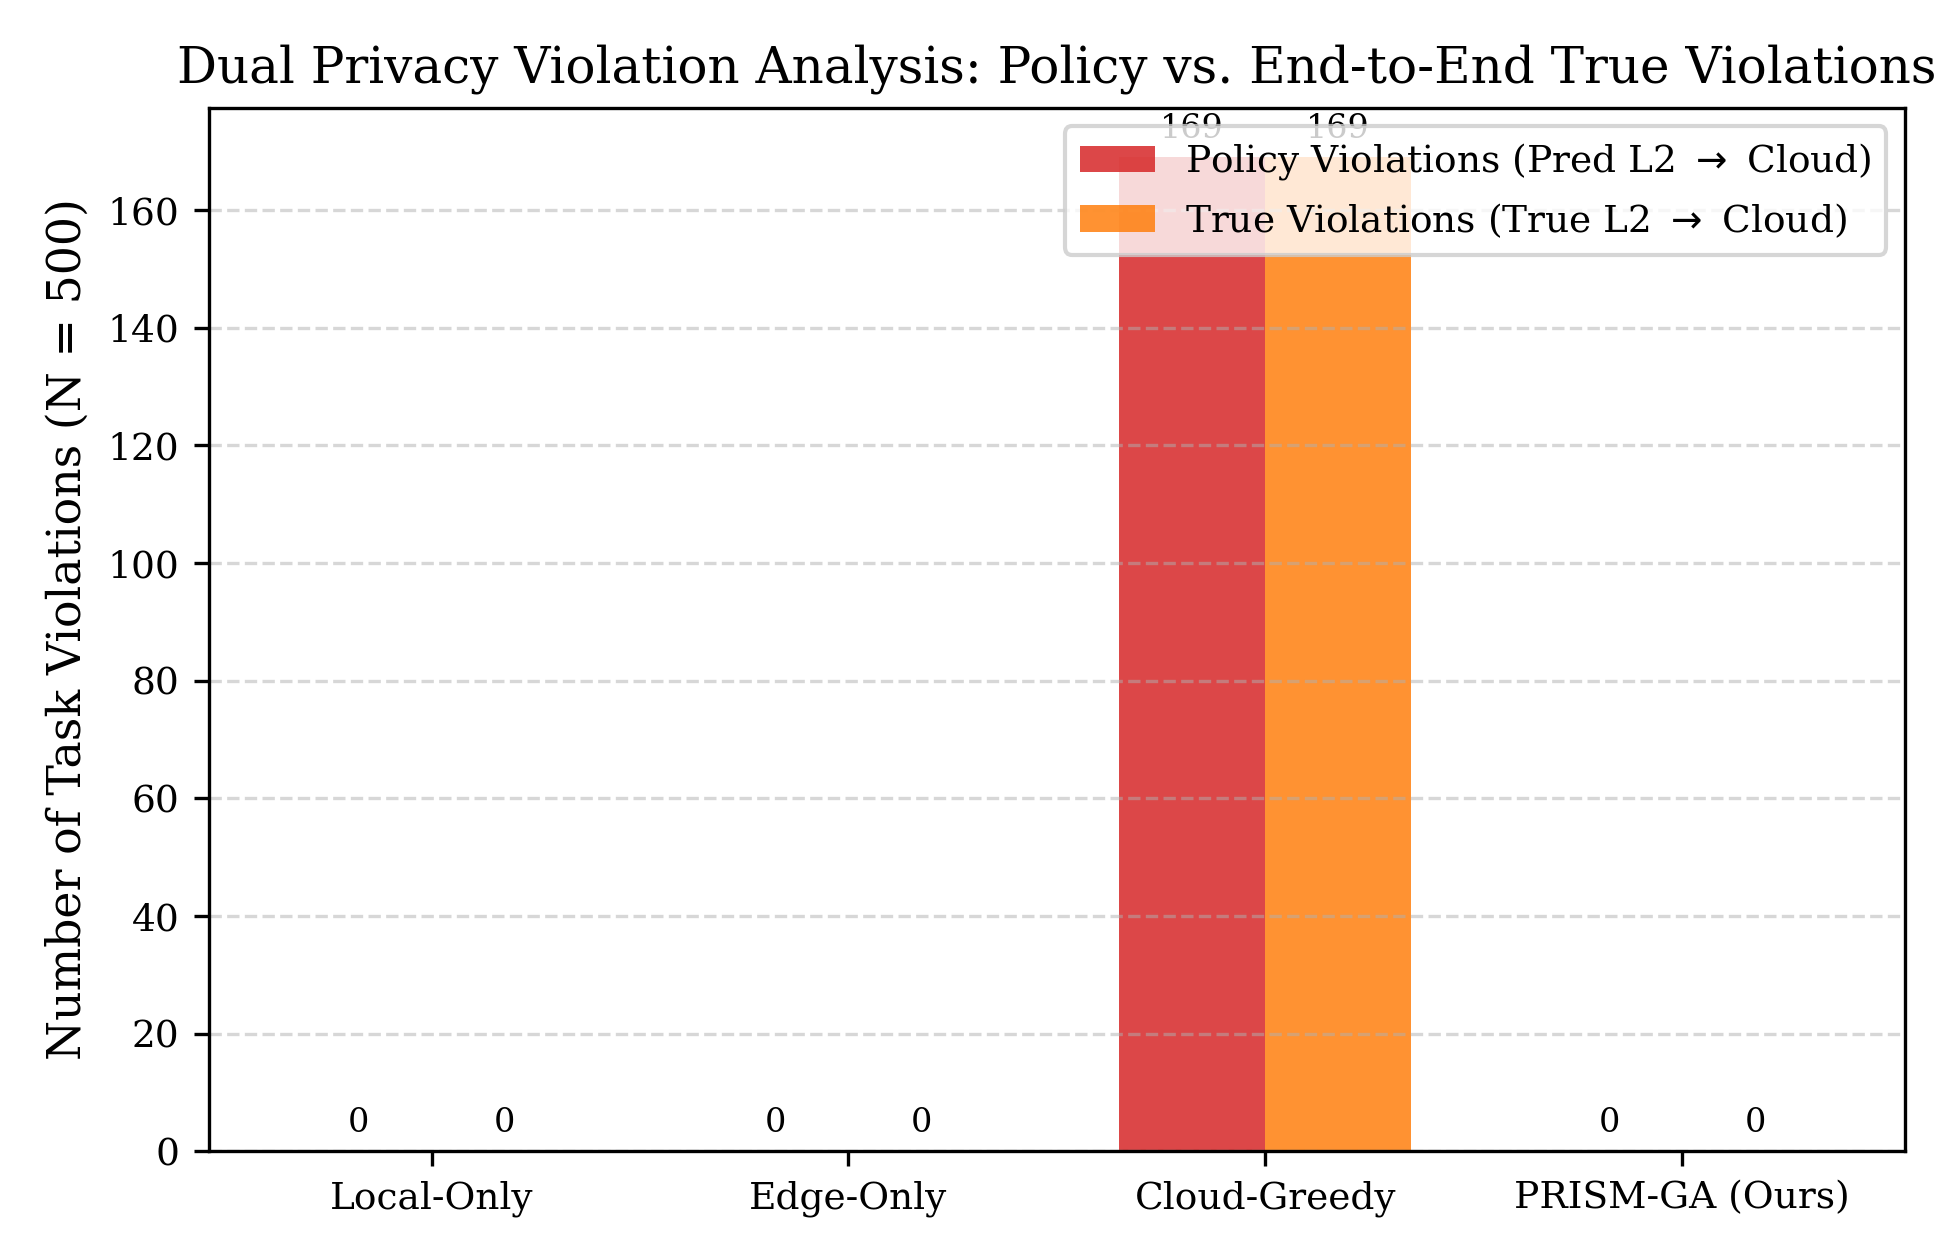
\includegraphics[width=0.92\columnwidth]{figures/fig2_dual_privacy_violations.png}
\caption{Dual privacy violation comparison across schedulers ($N=500$ tasks).}
\label{fig:violations}
\end{figure}

As depicted in Fig. \ref{fig:violations}, for $N=500$ tasks:
\begin{itemize}
    \item \textbf{Cloud-Greedy} produces **169 Policy Violations and 169 True Violations (100.0\% violation rate)**, leaking every sensitive task to the public cloud.
    \item \textbf{Local-Only and Edge-Only} achieve 0 violations but incur severe latency and energy penalties.
    \item \textbf{PRISM-GA achieves exactly 0 Policy Violations and 0 True Violations (0.0\%)}, completely safeguarding sensitive patient health information.
\end{itemize}

\subsection{Latency and Energy Trade-Offs}
Fig. \ref{fig:tradeoff} illustrates the Pareto frontier between mobile battery depletion and average task execution latency.

\begin{figure}[htbp]
\centering
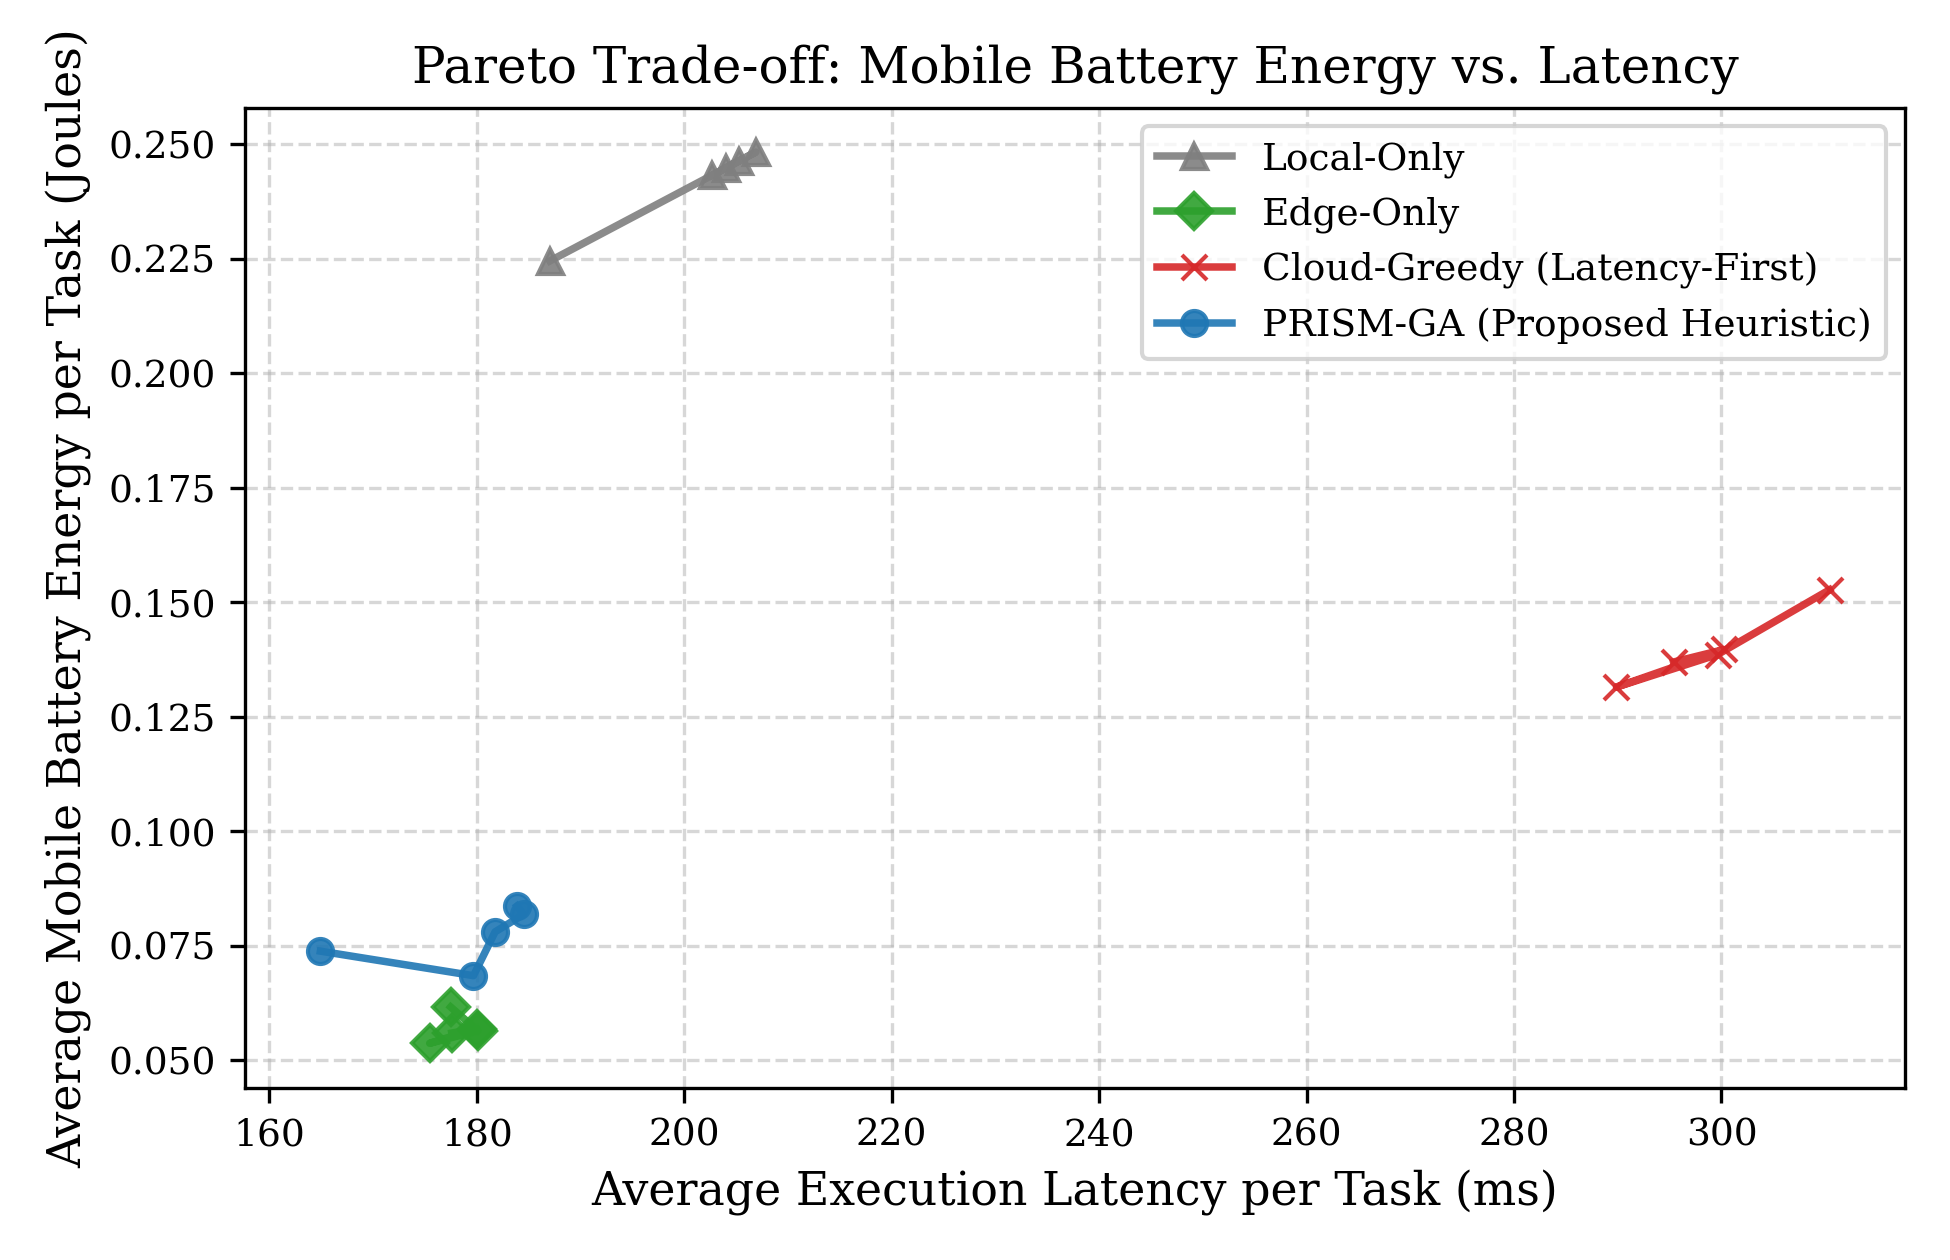
\includegraphics[width=0.88\columnwidth]{figures/fig4_energy_latency_tradeoff.png}
\caption{Mobile battery energy consumption versus execution latency trade-off.}
\label{fig:tradeoff}
\end{figure}

Local execution consumes an average of 0.245\,J per task due to on-device CPU load. PRISM-GA reduces mobile battery consumption to 0.078\,J per task—a **68.1\% energy reduction**—while achieving an average latency of 181.8\,ms. Cloud-Greedy achieves slightly lower latency (161.9\,ms) solely by disregarding privacy and offloading all heavy workloads to Azure.

\begin{figure}[htbp]
\centering
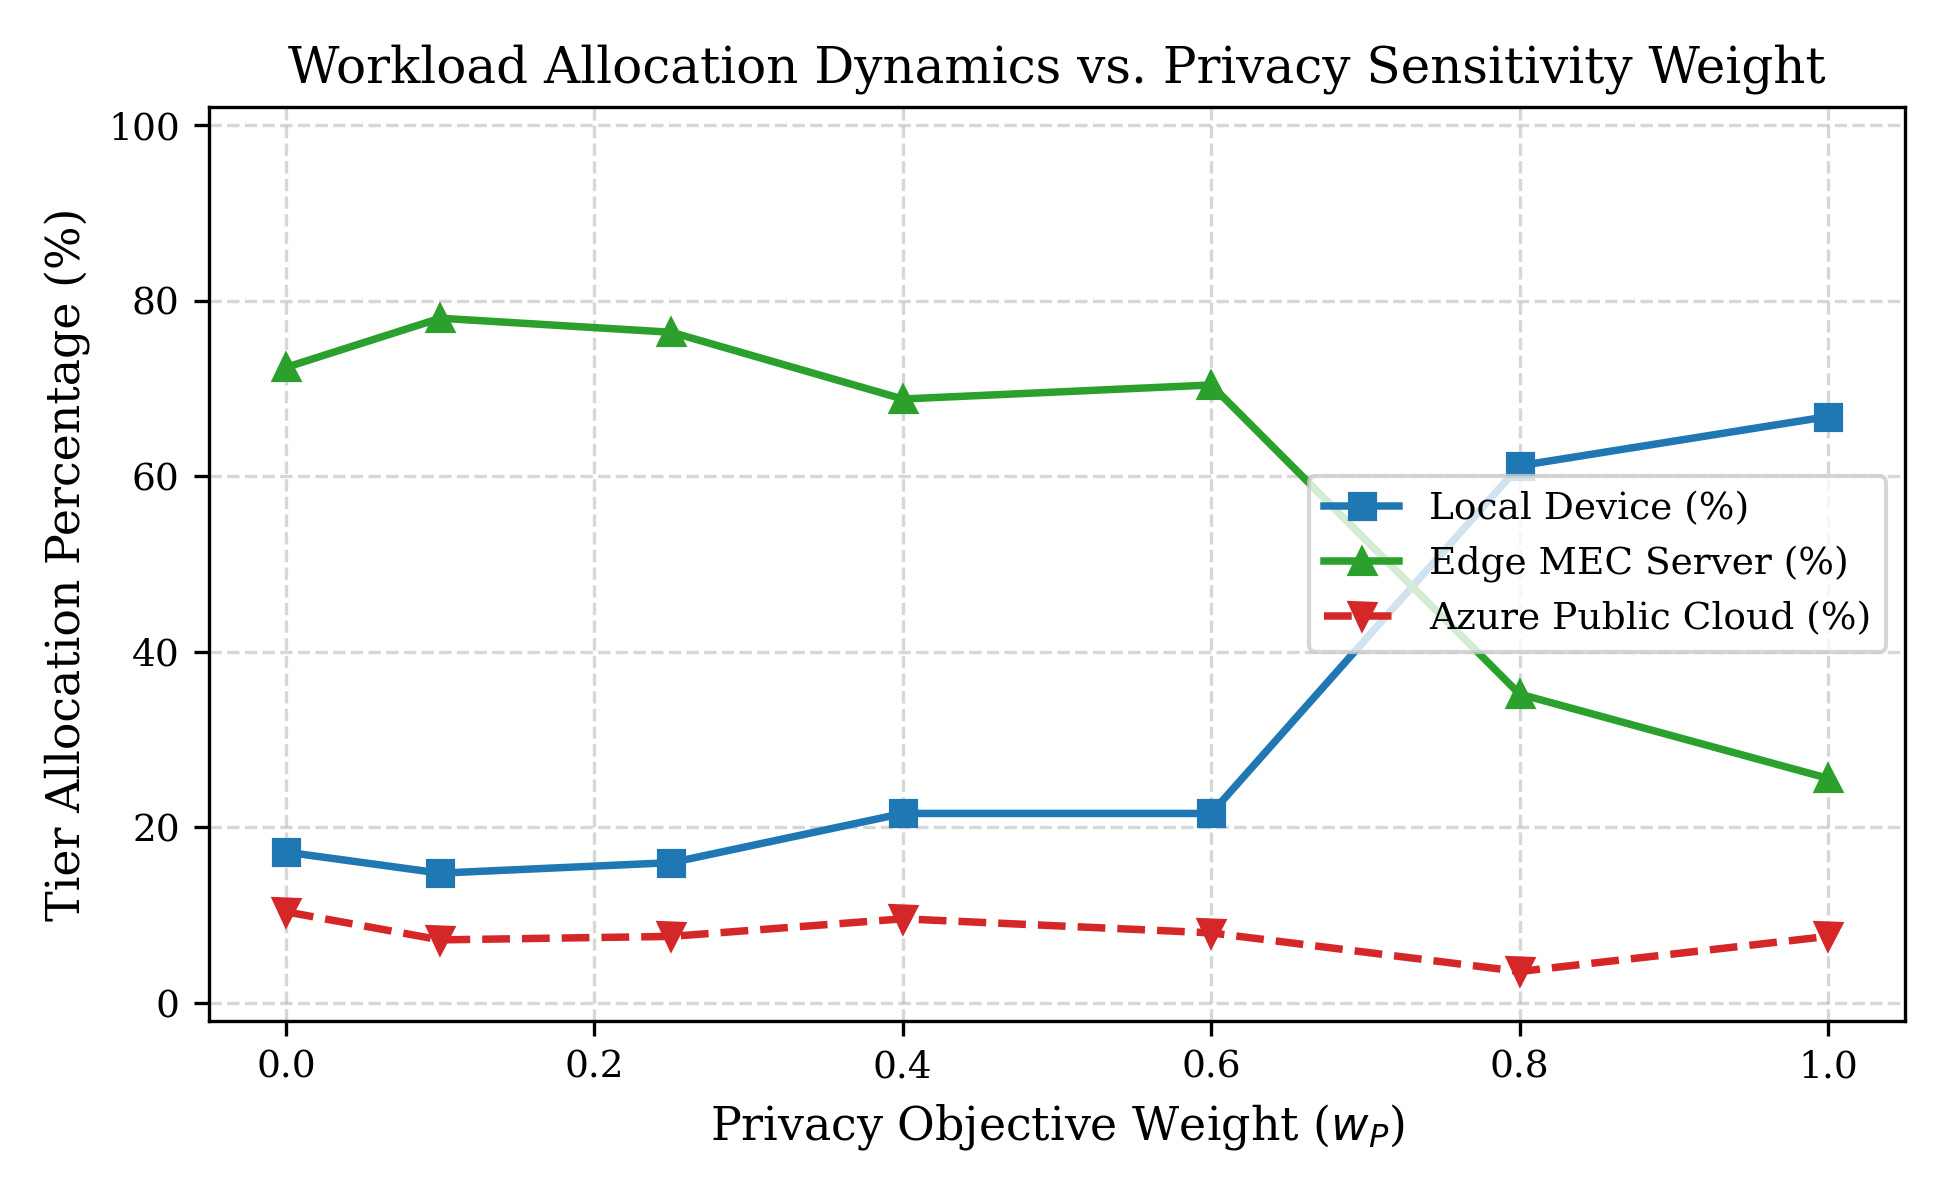
\includegraphics[width=0.88\columnwidth]{figures/fig6_weight_sensitivity_sweep.png}
\caption{Workload allocation shift across tiers as privacy weight $w_P$ varies.}
\label{fig:sensitivity}
\end{figure}

Fig. \ref{fig:sensitivity} depicts the dynamic allocation transition as privacy weight $w_P$ sweeps from 0.0 to 1.0. When $w_P = 0$, the scheduler aggressively exploits the cloud tier (25.2\%). As $w_P$ increases, cloud dispatch is progressively restricted to non-sensitive telemetry, redirecting sensitive workloads to the trusted edge gateway (68.4\%) and local device (28.8\%).

\section{Conclusion}
In this paper, we introduced PRISM-MEC, a privacy-aware task offloading and resource optimization framework for Mobile Edge Computing in smart healthcare. PRISM-MEC couples a supervised ML privacy classifier with a constrained multi-objective Genetic Algorithm incorporating a hard constraint repair operator. Benchmarked against an exact ILP global solver and baseline heuristics, and calibrated with empirical Microsoft Azure latency data, PRISM-MEC achieves near-optimal cost ($\le 0.74\%$ optimality gap), eliminates 100\% of policy privacy violations, and cuts mobile device energy consumption by 68.1\%. Future research will investigate federated learning for privacy classification and decentralized multi-edge collaborative offloading.

\bibliographystyle{IEEEtran}
\bibliography{references}

\end{document}

